\chapter{System Implementation and Evaluation}
\label{cha:system}
As we proposing methods to address different aspects of the research problems listed in Section \ref{sec:research_problem}, we implemented the partial solutions with some GUI and API, they can be used separately to solve each problem.
It's possible to integrate all components into one holistic framework, but since later parts were developed with more advanced technologies, integrating with older implementations makes it inefficient. So we presented those solutions as it is.

\section{CoCoOn Websites and Services}
\label{sec:cocoonImplementation}
This data model has evolved over time with the Cloud Service landscape.
We started the model with taxonomy definitions of Cloud terminologies,
see Section \ref{sec:cocoon0.1}.
Then we extended part of the ontology and developed it into
a the current version 1.0, see Section \ref{sec:cocoon1.0.1}.

The details of CoCoOn is described in Chapter \ref{cha:cocoon}. This section will explain how to use and make extension to the ontology, including: How are the ontologies, documentation, datasets hosted? How data can be collected and transformed with this ontology? How to query the result with SPARQL? And some other usage cases.

\subsection{Ontology Usage Cases}
\href{https://schema.org/}{Schema.org} does not formally include any Cloud Computing ontology yet, CoCoOn can be an extension in this area.
Its intended usage is illustrated in Figure \ref{fig:cocoon_workflow}.

\begin{figure}[!ht]
  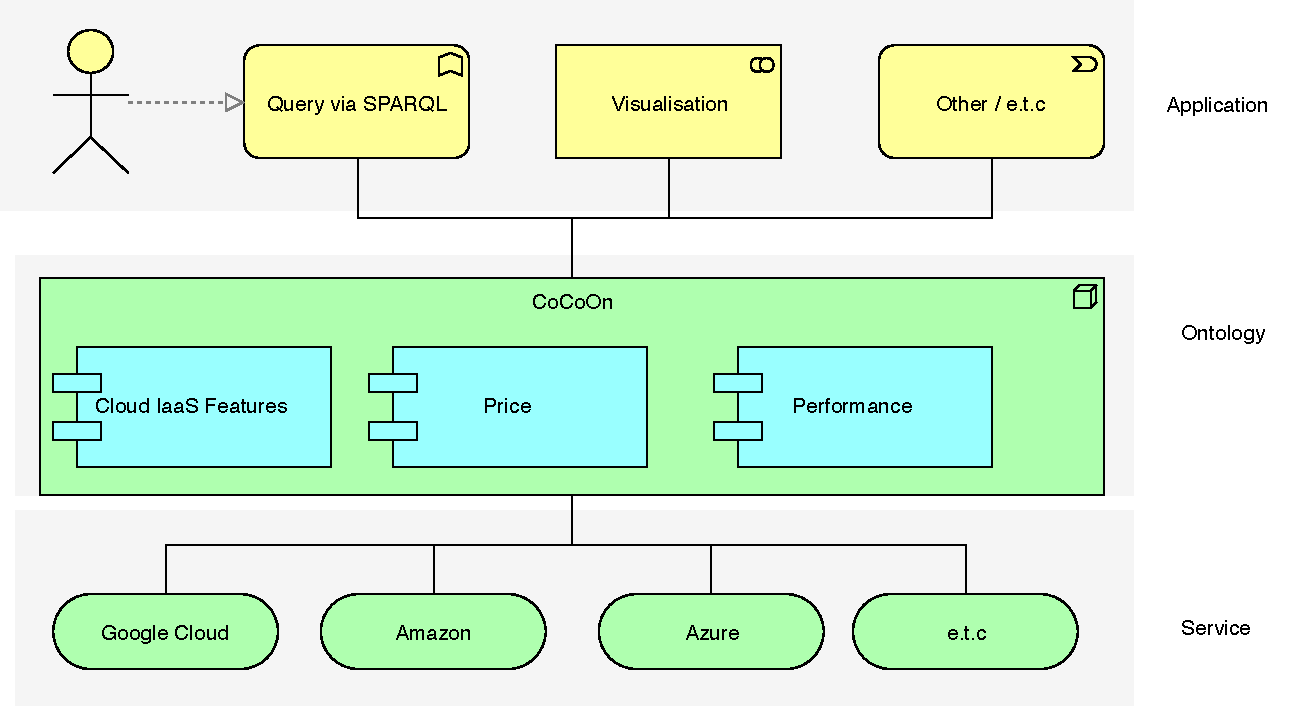
\includegraphics[width=\textwidth,keepaspectratio]{Figures/system/cocoon_usecase.pdf}
  \caption{CoCoOn Workflow}
  \label{fig:cocoon_workflow}
\end{figure}

\subsection{Mapping Data to Ontology}
For converting data from various sources to semantic data,
a number of methods were explored.
Initially we tried to transform the JSON file from the Provider APIs into a JSON-LD file by adding a \texttt{@context} to it.
After \href{https://miranda-zhang.github.io/cloud-computing-schema/json-ld-macros/gcloud.html}{experimenting with JSON-LD Macros} \cite{json-ld-macros}, we realized there are many limitations.
It only works well for simple cases but it is not sufficient to cover more complex scenarios.
So we moved to use SPARQL-Generate \cite{lefrancois_eswc_2017,sparql-generate}
for defining the mappings.

\subsubsection{Data Clean Up}
A lot of the data can be obtained from provider APIs,
in JSON or JS format.
We then clean up/transform such data with \href{https://stedolan.github.io/jq/}{jq}.
Next we mapped the cleaner data to ontologies,
and get results in RDF turtle format.

An example jq script transforms
\href{https://cloudpricingcalculator.appspot.com/static/data/pricelist.json}{json data from Google API}
is illustrated in Listing \ref{lst:jqScriptTransformsDataFromGoogleAPI}.
The \href{https://github.com/miranda-zhang/cloud-computing-schema/blob/master/example/gcloud/compute.md}{complete process with input and output} for each step is documented online with more details.

% I don't have a syntax highlighting setting for jq, so just used bash.
\begin{lstlisting}[caption={jq script transforms data from Google API},label={lst:jqScriptTransformsDataFromGoogleAPI},language=bash]
.gcp_price_list | . |=with_entries(select(.key| contains("VMIMAGE") )) | 
[ to_entries[] | 
    {
        "name": .key,
        "cores":(
            if (.key|contains("F1-MICRO")) then
                0.2 
            elif (.key|contains("G1-SMALL")) then
                0.5
            else .value.cores end
        ),
        "memory": .value.memory,
        "gceu": (
            if .value.gceu == "Shared CPU, not guaranteed" then
                null
            else .value.gceu end
        ),
        "maxNumberOfPd": .value.maxNumberOfPd,
        "maxPdSize": .value.maxPdSize,
        "price": 
         [ 
            .value | del(
                .cores, .memory, .gceu,
                .fixed, .maxNumberOfPd, .maxPdSize, .ssd)
            | to_entries[] | { "region": .key, "price": .value }
         ] 
    } 
]
\end{lstlisting}

\subsubsection{Annotating Plain Data with CoCoOn}
An example SPARQL-Generate script maps 
\href{https://azure.microsoft.com/api/v2/pricing/managed-disks/calculator/?culture=en-au&discount=mosp}{json data from Azure API about managed-disks}
to CoCoOn v1.0.1 is illustrated in Listing \ref{lst:rqgScriptAzureManaged-disks}.
The \href{https://github.com/miranda-zhang/cloud-computing-schema/blob/master/example/azure/storage.md}{complete process with input output} for each step is documented online with more details.

\begin{lstlisting}[caption={SPARQL-Generate script maps json data to ontologies},label={lst:rqgScriptAzureManaged-disks},language=sparql]
BASE <https://w3id.org/cocoon/data/v1.0.1/>
PREFIX iter: <http://w3id.org/sparql-generate/iter/>
PREFIX fun: <http://w3id.org/sparql-generate/fn/>
PREFIX rdfs: <http://www.w3.org/2000/01/rdf-schema#>
PREFIX xsd: <http://www.w3.org/2001/XMLSchema#>
PREFIX gr: <http://purl.org/goodrelations/v1#>
PREFIX cocoon: <http://w3id.org/cocoon/v1.0.1#>
PREFIX schema: <https://schema.org/>
PREFIX unit: <http://qudt.org/1.1/vocab/unit#>

GENERATE { 
  ?iri a cocoon:NetworkStorage;
    rdfs:label ?name;
    schema:dateModified ?date;
    cocoon:hasProvider ?provider;
    
    GENERATE {
        ?iri gr:hasPriceSpecification [ 
            a gr:CloudServicePriceSpecification ; 
                gr:hasCurrency "USD"^^xsd:string; 
                gr:hasCurrencyValue ?value;
                gr:hasUnitOfMeasurement cocoon:GBPerMonth ;
                cocoon:inRegion <Region/{?provider_slug}/{?region}>;
        ]
    }
  	ITERATOR iter:JSONListKeys(?prices) AS ?region
    WHERE {
        FILTER( ! CONTAINS(?managed_disk,"ultrassd") )
        BIND (xsd:float( fun:JSONPath(?prices,"$.['{?region}'].value") ) AS ?value )
    } .

    GENERATE {
        ?iri
        cocoon:hasStorageIOMax [
            a schema:TypeAndQuantityNode;
                schema:amountOfThisGood ?iops;
                schema:unitCode cocoon:IOPs;
        ];
        cocoon:hasStorageSize [
            a schema:TypeAndQuantityNode;
                schema:amountOfThisGood ?size;
                schema:unitCode cocoon:GB;
        ];
        cocoon:hasStorageThroughputMax [
            a schema:TypeAndQuantityNode;
                schema:amountOfThisGood ?speed;
                schema:unitCode unit:MegabitsPerSecond ;
        ];
    } WHERE {
        BIND (xsd:nonNegativeInteger( fun:JSONPath(?managed_disk_json,"$.iops") ) AS ?iops )
        BIND (xsd:nonNegativeInteger( fun:JSONPath(?managed_disk_json,"$.size") ) AS ?size)
        BIND (xsd:nonNegativeInteger( fun:JSONPath(?managed_disk_json,"$.speed") ) AS ?speed)        
        FILTER( BOUND(?iops) )
        # either ?iops ?size ?speed are all bound or non is bound
    } .

    GENERATE {
        ?iri
            gr:hasPriceSpecification <{?updated}/CloudStorageTransactionsPriceSpecification/{?provider_slug}/managed_disk/transactions-{?type}>;
    } WHERE {
        FILTER( ! CONTAINS(?managed_disk,"snapshot") && ! CONTAINS(?managed_disk,"ultrassd"))
        FILTER( CONTAINS(?managed_disk,"hdd") || CONTAINS(?managed_disk,"ssd") )
        BIND ( IF( CONTAINS(?managed_disk,"hdd") , "hdd" ,"ssd" ) AS ?type )        
    } .

    GENERATE {
        ?iri
            cocoon:canHaveSnapshot <{?updated}/NetworkStorage/{?provider_slug}/standardssd-snapshot>;
            cocoon:canHaveSnapshot <{?updated}/NetworkStorage/{?provider_slug}/standardhdd-snapshot-lrs>;
            cocoon:canHaveSnapshot <{?updated}/NetworkStorage/{?provider_slug}/standardhdd-snapshot-zrs>;
            cocoon:canHaveSnapshot <{?updated}/NetworkStorage/{?provider_slug}/{?premiumssd_snapshot}>;
    } WHERE {
        FILTER( !CONTAINS(?managed_disk,"snapshot") )
        FILTER( CONTAINS(?managed_disk,"premiumssd") || CONTAINS(?managed_disk,"standardssd"))
        BIND ( IF( CONTAINS(?managed_disk, "premiumssd") , "premiumssd-snapshot" , ?undefined ) AS ?premiumssd_snapshot )    
    } .

    GENERATE {
        ?iri gr:hasPriceSpecification [ 
            a gr:CloudServicePriceSpecification ;
                gr:hasCurrency "USD"^^xsd:string; 
                gr:hasCurrencyValue ?value;
                gr:hasUnitOfMeasurement ?unit ;
                cocoon:inRegion <Region/{?provider_slug}/{?region}>;
                rdfs:label ?label;
        ].
    }
  	ITERATOR iter:JSONListKeys(?prices) AS ?region
    WHERE {
        FILTER( CONTAINS(?managed_disk,"ultrassd") ) 
        BIND (xsd:float( fun:JSONPath(?prices,"$.['{?region}'].value") ) AS ?value )
        BIND (
            COALESCE(
                IF(CONTAINS(?managed_disk,"iops"), cocoon:IOPsPerHour, 1/0),
                IF(CONTAINS(?managed_disk,"stored"), cocoon:GBPerHour, 1/0),
                IF(CONTAINS(?managed_disk,"throughput"), cocoon:MegabitsPerSecondPerHour, 1/0),
                cocoon:VcpuPerHour # assume "vcpu"
            ) AS ?unit
        )
        BIND ( STRAFTER(?managed_disk,"-") AS ?label)      
    } .
}
SOURCE <https://raw.githubusercontent.com/miranda-zhang/cloud-computing-schema/master/example/jq/azure/2019-03-07/managed-disks.json> AS ?source
ITERATOR iter:JSONListKeys(?source) AS ?managed_disk
WHERE {
    BIND (fun:JSONPath(?source,"$.['{?managed_disk}']") AS ?managed_disk_json)
    BIND (fun:JSONPath(?managed_disk_json,"$.prices") AS ?prices)
    # having signle point of change for the following
    BIND ( "Azure" as ?provider_slug )
    BIND ( cocoon:Azure as ?provider )
    BIND ( "2019-03-07" as ?updated) # yr-month-day
    BIND ( xsd:date(?updated) as ?date )
    BIND ( IF (CONTAINS(?managed_disk,"ultrassd"), "ultrassd", ?managed_disk) AS ?name )
    BIND ( <{?updated}/NetworkStorage/{?provider_slug}/{?name}> AS ?iri )
}
\end{lstlisting}

\href{https://github.com/miranda-zhang/cloud-computing-schema/tree/master/example/sparql-generate}{More examples are online}. For those scripted tasks, we can automate the process, and additional information collection steps with human interpretation mostly are once off task which we have addressed with this project.

\subsubsection{Result}
We have also made the complete data-set (132,282 triples) available at
\href{https://w3id.org/cocoon/data}{https://w3id.org/cocoon/data}.
It is hosted with \href{http://linkeddatafragments.org/}{Linked Data Fragments Server} on Google Cloud.

\section{QoS Profiler}
In this section we describe the implementation of this QoS profiler proposed in Section \ref{sec:qos}.

\subsection{QoS Data Collection Scripts}
Data is collected from \href{https://cloudharmony.com}{CloudHarmony}, initially we used the HtmlUnit library \cite{htmlunit}.

Later as CloudHarmony evolves, we also upgraded our script.
\href{https://github.com/miranda-zhang/cloud-computing-schema/tree/master/example/cloudharmony}{More technical details on measuring QoS} is documented online. We also provided live demos of QoS tests, e.g.
\href{https://miranda-zhang.github.io/cloud-computing-schema/cloudharmony/google/test.html}{Downlink Speed and Latency tests for Google Cloud Services}.
\href{https://github.com/miranda-zhang/cloud-computing-schema/blob/master/example/cloudharmony/selenium/cloudharmony.py}{Uplink tests scripts are written in python}
as \href{https://github.com/miranda-zhang/cloud-computing-schema/tree/master/example/cloudharmony/selenium}{selenium} is required.

\subsection{Distributed Archetecture}
Fig. \ref{fig1} shows the top level dataflow of the system we implemented.

\begin{figure}[!ht]
 \centering
 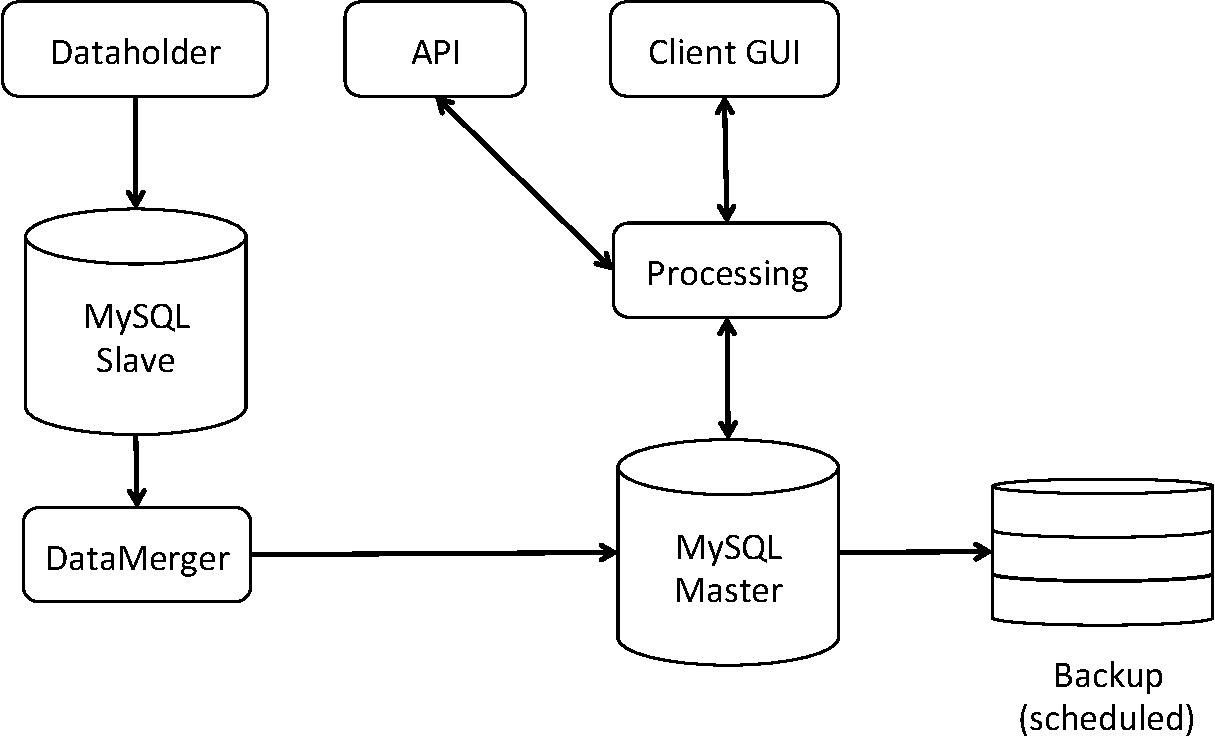
\includegraphics[width=\textwidth,keepaspectratio]{Figures/QoS/figure1.pdf}
 \caption{Abstract System Dataflow. This figure is better looking together with Fig. \ref{fig:QoSMonitoringServiceNetworkTopology} for better understanding. As we have used several (slave) servers to collect data from different locations. Then we transfer them to a central server for processing and backup, data on this server was also archived and cleared manually every time after we imported the newly collected data into the local offline system for post-processing and cleaning up. We only use the (summarised) average QoS data for real time querying via API and web GUI, as this allows us to provide response faster.}
\label{fig1}
\end{figure}

Fig. \ref{fig3} shows the overview of our system architecture. We use Dropbox as the backup service for this prototype implementation to demonstrate the feasibility. As long as data is properly backed up in a separate location, other mechanisms can be used, i.e. git repository.

\begin{figure}[!ht]
 \centering
 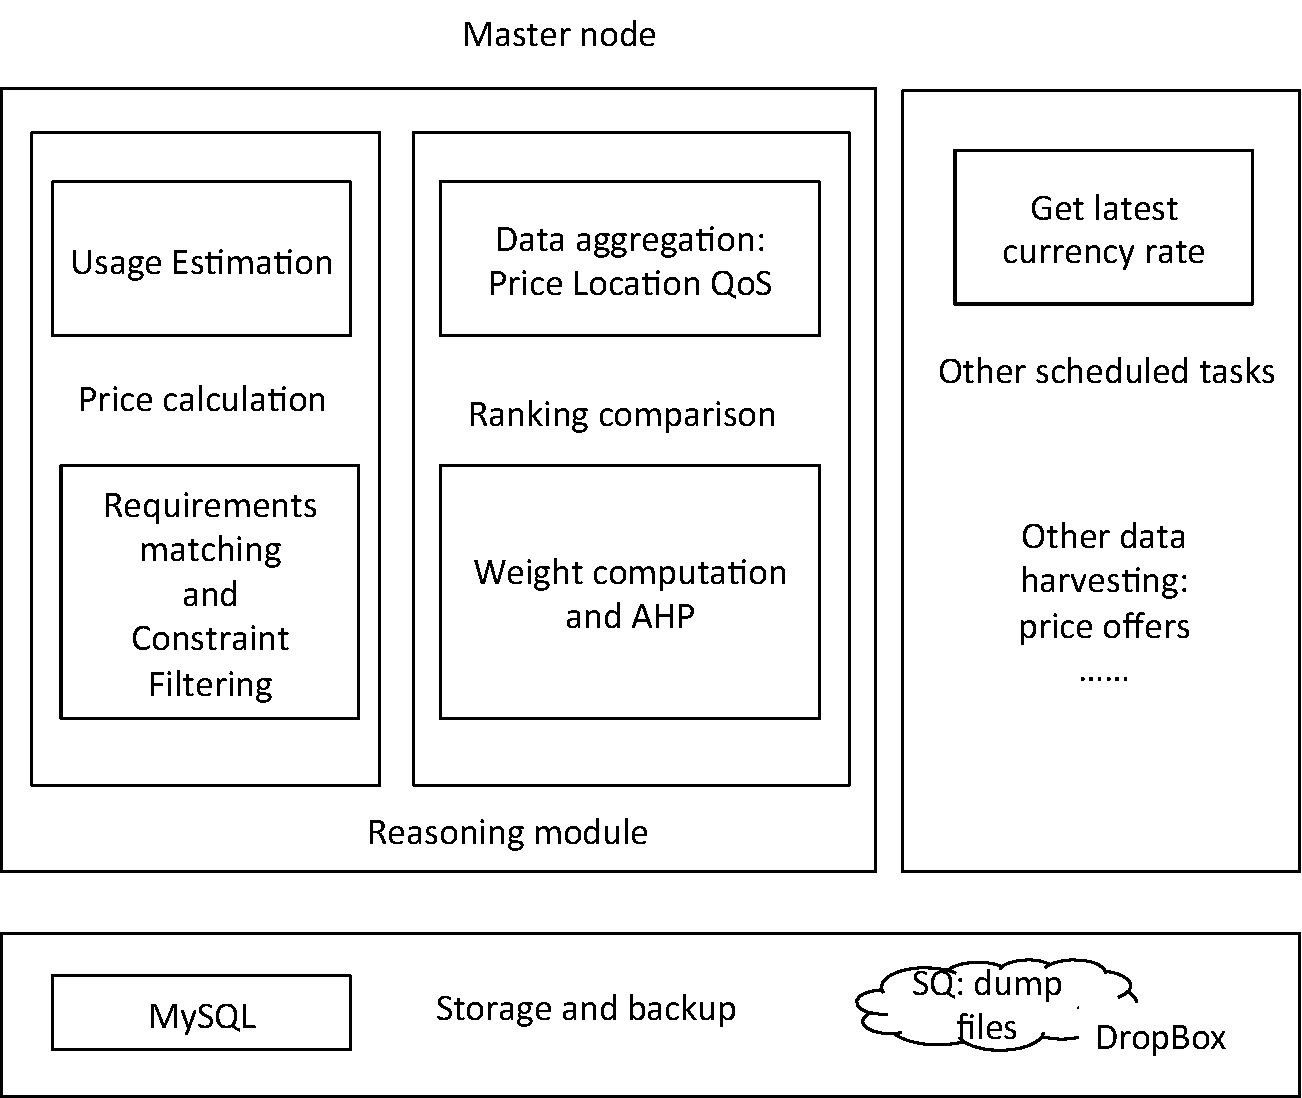
\includegraphics[width=\textwidth,keepaspectratio]{Figures/QoS/figure3.pdf}
 \caption{Master Node System Architecture. In the reasoning module main functions and operations are broke down into different blocks. There are some other tasks cannot be strictly categorized into existing modules, those are put into the ``Other Tasks" section, and the very light grey block contains the evolving part of the system so it cannot be considered a stable component of the system. While it’s possible to backup the whole server, it is not necessary at this stage, and the most valuable data is stored in the MySQL database, which can be backuped much easier and cheaper by creating ``SQL dump". This dump file is created daily and simply stored in a Dropbox folder which is free to use and keeps a history of the file stored in it for 30 days, which is sufficient for our case. The presentation layer (UI and API implementation) and monitoring module are omitted to keep the diagram simple.}
\label{fig3}
\end{figure}

The price data is collected from providers' websites. The problem with automatic data collection can be solved if providers release more structured data with sufficient metadata description, we have proposed an ontology in Chapter \ref{cha:cocoon}.

\section{CloudRecommender}
\label{sec:CloudRecommender}
Despite the popularity of Cloud Computing, existing Cloud Service manipulations (e.g. select, start, stop, configure, delete, scale and de-scale) techniques require human familiarity with different Cloud service types and typically rely on procedural programming or scripting languages. The interaction with services is performed through low-level application programming interfaces (APIs) and command line interfaces. This is inadequate, given the proliferation of new providers offering services at different layers (e.g. SaaS, PaaS, and IaaS). One of the consequences of this state is that accessibility to Cloud Computing is limited to decision makers with IT expertise. This raises a set of research questions: How to develop interfaces that can transform low, system-level programming to easy-to-use drag and drop operations? Will such interfaces improve and simplify the process of Cloud Service Selection and Comparison?

Therefore, we present CloudRecommender, a decision support system, using transactional SQL semantics, procedures and views. The benefits to users of CloudRecommender include, for example, the ability to estimate costs, compute cost savings across multiple providers with possible tradeoffs and provide visual aid in the selection of Cloud services.

\subsection{Related Work}
Prior to CloudRecommender, there have been a variety of systems that use declarative logic-based techniques for managing resources in distributed computing systems. The focus of the authors in work \cite{Liu2011} is to provide a distributed platform that enables Cloud providers to automate the process of service orchestration via the use of declarative policy languages.
The authors in \cite{Brodsky2009} present an SQL-based decision query language for providing a high-level abstraction for expressing decision guidance problems in an intuitive manner so that database programmers can use mathematical programming technique without prior experience.
We also draw inspiration from the work in \cite{DBLPconfCIDRMaoLMF11} which proposes a data-centric (declarative) framework to improve SLA fulfillment ability of Cloud service providers by dynamically relocating infrastructure services.
COOLDAID \cite{Chen2010} presents a declarative approach to manage configuration of network devices and adopts a relational data model and Datalog-style query language.
NetDB \cite{Caldwell2004} uses a relational database to manage the configurations of network devices. However, NetDB is a data warehouse, not designed for Cloud service selection or comparison. However, NetDB is a data warehouse, not designed for Cloud service selection or comparison. 

In contrast to the aforementioned approaches, CloudRecommender is designed for solving the new challenge of handling heterogeneous service configuration and naming conventions in Cloud computing. It is designed with a different application domain – one that aims to apply declarative and widget programming technique for solving the Cloud service selection problem.

\subsection{System Architecture}
The CloudRecommender system architecture consists of three layers: the configuration management layer, the application logic layer and the User interface (widget) layer.
Shown in Fig. \ref{fig:SystemDeploymentStructure}.

\begin{figure}[!ht]
  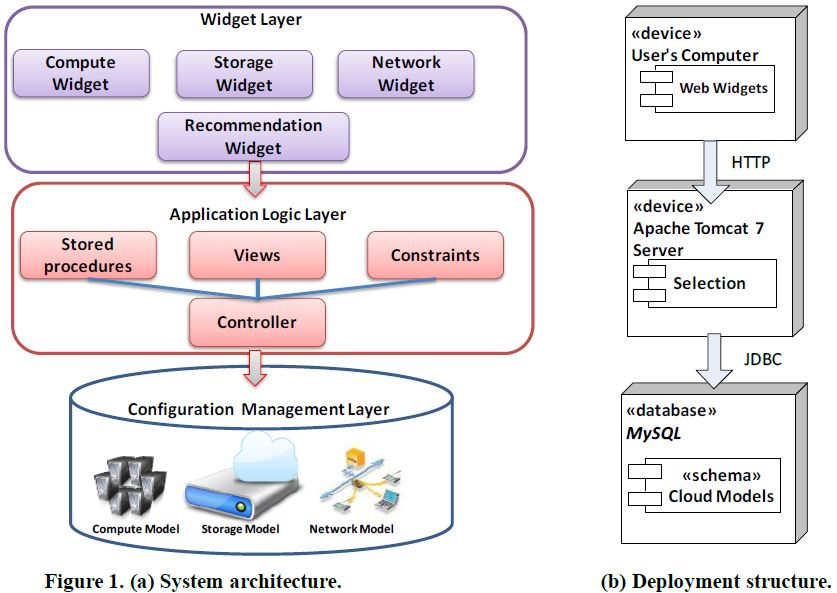
\includegraphics[width=\textwidth,keepaspectratio]{Figures/system/CloudRecommender/SystemArchitecture.jpg}
  \caption{System architecture and deployment structure}
  \label{fig:SystemDeploymentStructure}
\end{figure}

Figure \ref{fig:SystemDeploymentStructure}(b) shows the deployment structure of the CloudRecommender system.
For persistence we have chosen MySQL for its agility and popularity, but any other relational database can be plugged in. 
Furthermore, many APIs provided by cloud
providers (such as Amazon) and open source cloud management frameworks (e.g.
jclouds) are written in Java. Thus, Java is chosen as the preferred language to
implement the application logic layer to ease the integration with external libraries.

The configuration layer maintains the basic cloud domain model related to compute, storage, and network services.
Initially we stored recommender system data into a relational database,
its implementation is detailed in Section \ref{sec:InfrastructureServiceConfigurationRepository}.
But as we go deeper with understanding of the Cloud domain,
we increasing find this database model is hard to update,
thus hard to keep up to date with rapid changing Cloud services,
and not very readable to whom do not have knowledge of our recommender system,
as the database schema designed to be optimal for recommendation service with unique table structure and procedures.
So later, we developed the Cloud Computing Ontology (CoCoOn) model with OWL.
See Chapter \ref{cha:cocoon}.
The later proposed model is flexible and extensible enough to accommodate new services with minimal changes to our implementation. 

\subsubsection{Configuration Management Layer}
\label{sec:InfrastructureServiceConfigurationRepository}
The repository of available infrastructure services from different
providers consists data of compute, storage and network services.
These infrastructure services have very different configurations and pricing models, see Section \ref{sec:TheProblemOfSelectingOptimalServiceConfiguration} for some examples.
We collected service configuration information from a
number of public cloud providers (e.g., Windows Azure, Amazon, GoGrid,
RackSpace, Nirvanix, Ninefold, SoftLayer, AT and T Synaptic, Cloud Central, etc.) to demonstrate the generic nature of the domain model with respect to capturing heterogeneous configuration information of infrastructure services. 

We formally capture the domain knowledge (e.g., IaaS configurations)
using a declarative logic-based language, and then apply the
knowledge on top of relational data model that encapsulates
Cloud-wide information. Based on this knowledge, we have
drawn the relationships in the conceptual IaaS configuration
model and represented in Fig. \ref{fig:uml}.

Relationships between concepts representing services are carefully considered and normalized to avoid update anomalies. Services from various providers often have very different configurations and pricing models. Distinct and ambiguous
terminologies are often used to describe similar configurations.
Regardless of how providers name their services, we categorize infrastructure services based on their basic functionality.
Unit conversions were performed during instantiation of concepts.

The choice of a relational model and SQL as query language was made because of the convenience SQL procedures offers us in regards to defining templates for a given widget type. We use stored procedures to create temporary tables and to concatenate parameters to dynamically generate queries based on the user input.

\begin{figure}
  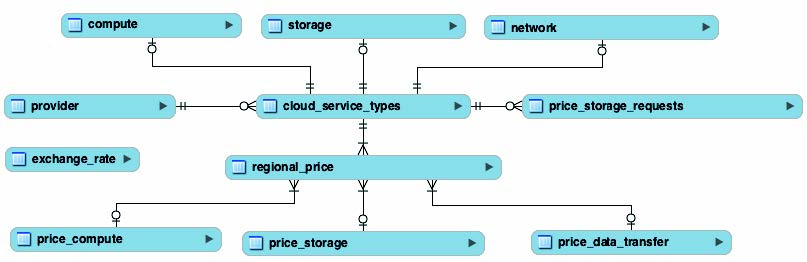
\includegraphics[width=\textwidth,keepaspectratio]{Figures/system/CloudRecommender/uml.jpg}
  \caption{Conceptual UML data model representing infrastructure service entities and their relationships}
  \label{fig:uml}
\end{figure}

For providers that offer different regional prices, we store the location information in the price table.
If multiple regions have the same price, we choose to combine them.
In the database version implementation, any changes to existing configurations (such as updating memory size, storage provision etc.) of services can be done by executing customized update SQL queries.

We have applied declarative service
selection technique by utilizing SQL and regular expressions
minimize side effects and reinforce constrains. Thus, leading
to a improved Cloud service representation and selection.

The service selection logic developed by our research is
transactional and applies well-defined SQL semantics for
querying, inserting, and updating IaaS configurations. In
addition, the proposed declarative approach is preferable
over hard coding the sorting and selection algorithm (as used
in \cite{Ruiz-AlvarezCloudStorageSelection})
as it allows us to take the advantage of optimized
query operations (e.g. select and join). 

The problem we are
trying to solve involves computing the Cartesian product
O(N * M) of multiple sets of options. A widely used solution
of such operation is the JOIN operation in database. Note
that much work in database-systems has aimed
at efficient implementation of joins. In fact, modern database
often use HASH JOIN O(N + M) and MERGE JOIN
O(N*Log(N) + M*Log(M)). They are much faster than O(N
* M).

\subsubsection{Application Logic Layer}
The request for service selection in CloudRecommender is expressed as SQL queries.
The selection process supports an application logic that builds upon the following declarative constructs: criterion, views and stored procedures. The CloudRecommender builds upon SQL queries which are executed on top of the relational data model.

\textbf{Criterion:} Criterion is a quantitative or qualitative bound (minimum, maximum, equal) on the configuration parameters provided by a service. Cloud services’
configuration parameters and their range/values listed in
Table \ref{table:IaaSConfigurations} form the basis for
expressing selection goal and criteria (e.g., select a cheapest (goal) compute service where (criterion) 0<Ram<=20, 0<=local storage<=2040, number of hours to be used per month = 244). 
An example query is shown below in Fig. \ref{fig:ExampleQueryProcedure}:

\begin{table}
\begin{tabular}{|l|p{5.5cm}|p{5.5cm}|}
\hline
Service                  & Configurations Parameters                                         & Range/possible values                                         \\ \hline
\multirow{9}{*}{Compute} & Core                                                              & >=1                                                           \\ \cline{2-3} 
                         & CPUClockSpeed                                                     & >0                                                            \\ \cline{2-3} 
                         & hasMemory                                                         & >0                                                            \\ \cline{2-3} 
                         & hasCapacity                                                       & >=0                                                           \\ \cline{2-3} 
                         & Location                                                          & North America, South America, Africa, Europe, Asia, Australia \\ \cline{2-3} 
                         & CostPerPeriod                                                     & >= 0                                                          \\ \cline{2-3} 
                         & PeriodLength                                                      & >0                                                            \\ \cline{2-3} 
                         & CostOverLimit                                                     & >= 0                                                          \\ \cline{2-3} 
                         & PlanType                                                          & Pay As You Go, Prepaid                                        \\ \hline
\multirow{7}{*}{Storage} & StorageSizeMin                                                    & >= 0                                                          \\ \cline{2-3} 
                         & StorageSizeMax                                                    & > 0                                                           \\ \cline{2-3} 
                         & CostPerPeriod (e.g. Period = Month) (e.g. UnitOfMeasurement = GB) & >= 0                                                          \\ \cline{2-3} 
                         & Location                                                          & North America, South America, Africa, Europe, Asia, Australia \\ \cline{2-3} 
                         & RequestType                                                       & put, copy, post, list, get, delete, search                    \\ \cline{2-3} 
                         & CostPerRequest                                                    & >= 0                                                          \\ \cline{2-3} 
                         & PlanType                                                          & Pay As You Go, Prepaid, Reduced Redundancy                    \\ \hline
\multirow{2}{*}{Network} & CostDataTransferIn                                                & >=0                                                           \\ \cline{2-3} 
                         & CostDataTransferOut                                               & >=0                                                           \\ \hline
\end{tabular}
\caption{Infrastructure service types and their configurations}
\label{table:IaaSConfigurations}
\end{table}

\begin{figure}
  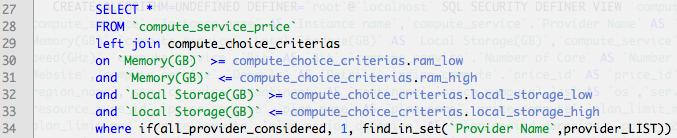
\includegraphics[width=\textwidth,keepaspectratio]{Figures/system/CloudRecommender/sql.jpg}
  \caption{Example query in procedure.}
  \label{fig:ExampleQueryProcedure}
\end{figure}

\textbf{Procedures:} We have implemented a number of customized procedures that automate the service selection process. A number of routines are prepared to process a user service selection request. List of inputs are stored in a temporary table to be passed into the procedures. As such, the size of the input list can be very long.
Final results are also stored in temporary tables, which are automatically cleared after the expiration of user session.

\textbf{Controller:} The controller supports enforcement of criteria and dynamically generates SQL queries which fulfill a given selection preference stated by the user.
Due to space considerations we are not able to depict the complete algorithm, but Fig. \ref{fig:SelectionLogic} shows the selection logic in a simplified diagram. Next we explain the basic
steps which are executed for resolving a service selection request.

\begin{figure}
  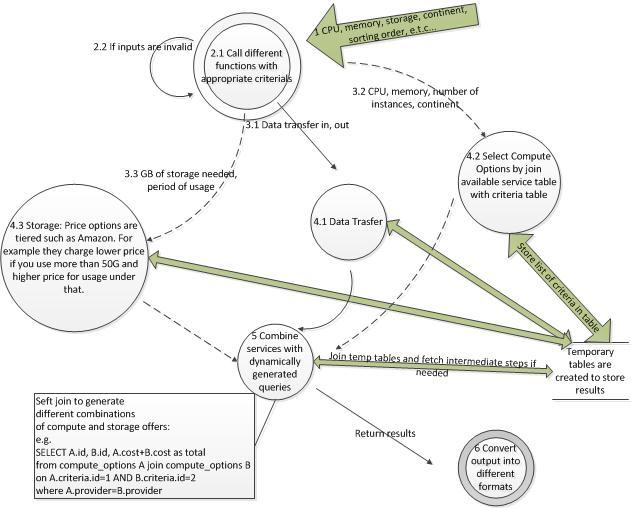
\includegraphics[width=\textwidth,keepaspectratio]{Figures/system/CloudRecommender/SelectionLogic.jpg}
  \caption{Service Selection logic.}
  \label{fig:SelectionLogic}
\end{figure}

\begin{enumerate}
    \item Basic validation is preformed on user inputs at the controller, appropriate errors are returned accordingly.
    \item Depending on user’s requirements, process 3.2 or 3.3 may not happen. This is why they are shown as dotted lines, i.e. user can query storage or compute only IaaS services. But data transfer parameters have to be set, as user will definitely transfer data in and out of the compute or storage service.
    \item Multiple temporary tables are created during the process so intermediate results (i.e. selection details of the final recommendation) can be fetched later as needed.
    \item It is possible for a user to choose multiple compute services each with different criteria. (E.g. they may have 10 set of requirements, and choose 10 instances for each.) So in process 5, query with different number of join operations are dynamically constructed.
    \item Currency conversions are performed before costs are compared.
\end{enumerate}

\textbf{Computational Complexity of Service Selection Logic}:
For a provider p, suppose it has r regions, v different kind of VMs,
s storage options, n network services.
There will be $r \times v$ different prices for VM, similarly for prices of storage ($r \times s$)
and network ($r \times n$).
And theoretically a total number of $r^{3} \times v \times s \times n$ possible combinations.
We can normally reduce the number of
options significantly in the early stage if a user has strict requirements. In the worst
case scenario, the logic needs to compute a full cross join (Cartesian product).

Another factor effecting the price calculation is the different price tiers for some services. 
Price tier example: AWS S3 charges 0.125 USD per GB for the first 1 TB /
month of usage, 0.093 for the next 49 TB, etc.
Depending on the estimated usage,
the larger the usage, the more price tiers will be involved.

Let us assume that each
provider offers approximately the same service in each region to simplify the
derivation of the computational complexity.

Let $cs_{p}$ be the number of compute services of provider p.
All regions are included, i.e. $cs_{p} = r \times v$.
Let $ss_{p}$ be the number of storage services, and $st_{p}$ be the number of storage service tiers,
$nt_{p}$ be the number of network service tiers,
$ns_{p}$ be the number of network services.
As such, the total number of offers can be
represented as follows:
$$
\sum_{p=1}^{P} cs_{p} \times (ss_{p} \times st_{p}) \times (ns_{p} \times nt_{p})
$$
Where P is the number of cloud providers.

The queries of the selection logic works as follows. After filtering out criteria-violating
services, resulting services are combined via JOIN operation(s) with final
costs calculated. In worst case scenario where a few or no criteria are defined, the
combination of the services is a full CROSS JOIN over all existing services.
Therefore, the selection queries, to our best knowledge,
have the upper bound computational complexity of
$$
O_{query}(\sum_{p=1}^{P}|cs_{p} c_{v} (ss_{p} st_{p} c_{s}) (ns_{p} nt_{p} c_{n}) | )
$$
where c means criteria, $c_{v}, c_{s}, c_{n}$ are criteria for compute, storage and network.
$ss_{p} st_{p}$ and $ns_{p} nt_{p}$ can be pre-computed, and stored as views.
However, in case the database system lacks
support for cached views in a worst case the effort multiplies with the effort of the
views’ JOIN. Modern database can use HASH JOIN O(N + M) and MERGE JOIN
O(N*Log(N) + M*Log(M)) which are faster than O(N * M).

\subsection{Interface: GUI and API}
The widget layer is implemented using a number of JavaScript frameworks including jQuery, ExtJS and YUI. CloudRecommender also exposes RESTful
(REpresentational State Transfer) APIs (application programming interface) that help external applications to programmatically compose infrastructure cloud services based on the CloudRecommender selection process.

\begin{figure}
  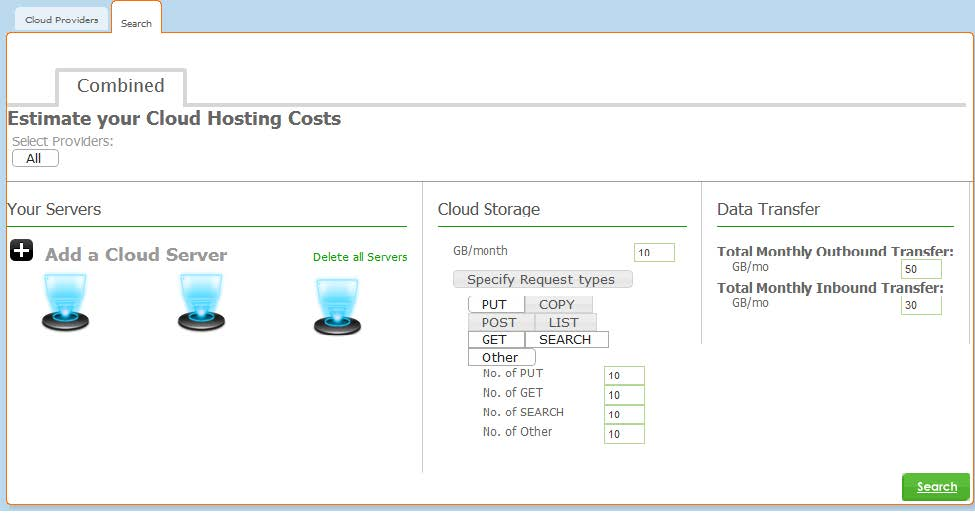
\includegraphics[width=\textwidth,keepaspectratio]{Figures/system/CloudRecommender/widget_combined.jpg}
  \caption{Screenshot of the widget combined tab.}
  \label{fig:widget_combined}
\end{figure}

\begin{figure}
  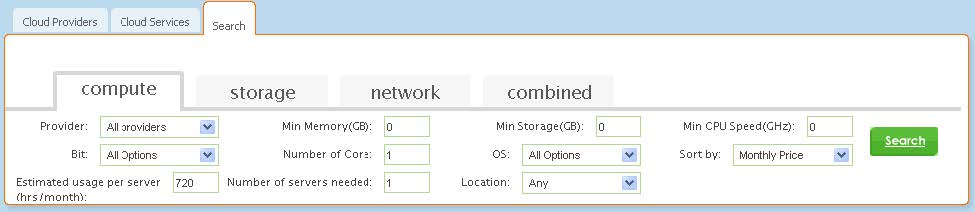
\includegraphics[width=\textwidth,keepaspectratio]{Figures/system/CloudRecommender/widget_compute.jpg}
  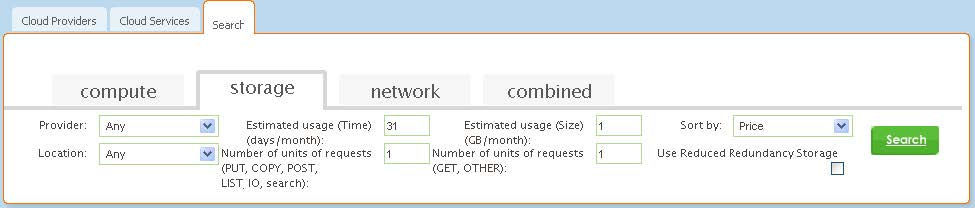
\includegraphics[width=\textwidth,keepaspectratio]{Figures/system/CloudRecommender/widget_storage.jpg}
  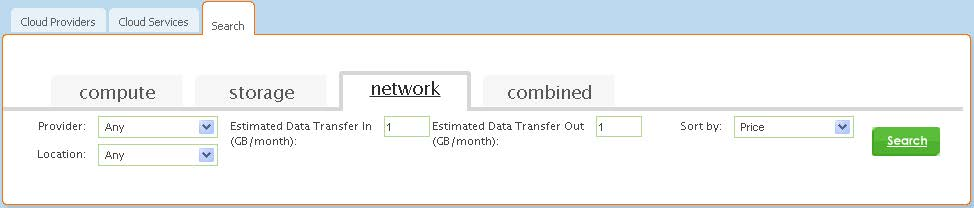
\includegraphics[width=\textwidth,keepaspectratio]{Figures/system/CloudRecommender/widget_network.jpg}
  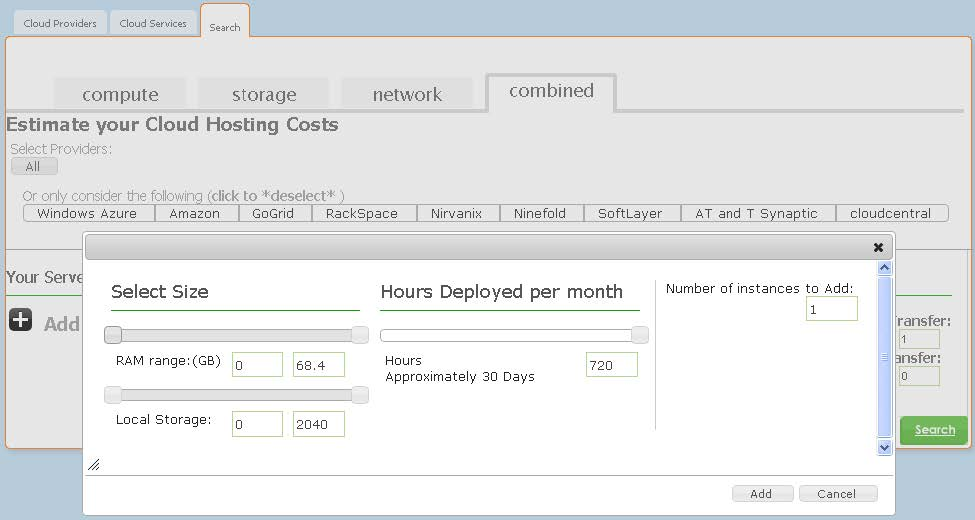
\includegraphics[width=\textwidth,keepaspectratio]{Figures/system/CloudRecommender/widget_combined_popup.jpg}
  \caption{Compute, Storage, Network and the combined service selection widgets screenshots.}
  \label{fig:widget_screenshots}
\end{figure}

This layer features rich set of user-interfaces (see Fig. \ref{fig:widget_combined}
and \ref{fig:widget_screenshots})
that further simplify the selection of configuration parameters related to cloud services.
This layer encapsulates the user interface components in the form of four principle widgets including: Compute, Storage, Network, and Recommendation. The selection of basic configuration parameters related to compute services including their RAM capacity, cores, and location can be facilitated through the Compute widget. It also allows users to search compute services by using regular expressions, sort by a specific column etc. Using the Compute widget, users can choose which columns to display and rearrange their order as well. The Storage widget allows users to define configuration parameters such as storage size and request types (e.g., get, put, post, copy, etc.). Service configuration parameters, such as the size of incoming data transfer and outgoing data transfer can be issued via the Network widget. Users have the option to select single service types as well as bundled (combined search) services driven by use cases. The selection results are displayed and can be browsed via the Recommendation widget.
See Section \ref{sec:case_studies} for some examples.

CloudRecommender also exposes REpresentational State
Transfer (RESTful) APIs that help external applications to
programmatically obtain results, i.e. recommended
infrastructure Cloud services configurations, shown in Fig. \ref{fig:REST}.

\begin{figure}[!ht]
  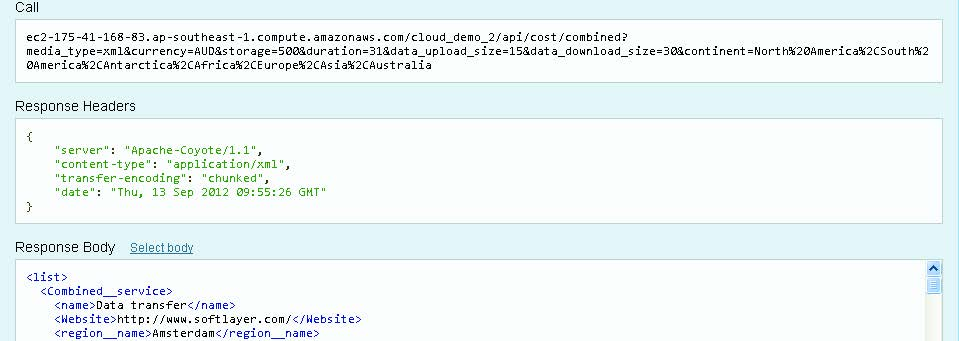
\includegraphics[width=\textwidth,keepaspectratio]{Figures/system/CloudRecommender/REST.jpg}
  \caption{REST call via HTTP GET request}
  \label{fig:REST}
\end{figure}

\subsection{Experiment}
In this section, we present the experiments and evaluation that we undertook.

\textbf{Experiment Setup:} We hosted our CloudRecommender system instance on Amazon
EC2 using a standard small instance in the US-west location. By default, the small
instance has the following hardware configuration: 1.7 GB of main memory, 1 EC2
Compute Unit, 160 GB of local instance storage, and a 32-bit platform with an
Ubuntu 10.04 operating system. We populated CloudRecommender with
infrastructure service configuration information related to Amazon, Azure, GoGrid,
RackSpace, Nirvanix, Ninefold, SoftLayer, AT and T Synaptic, and Cloud Central (an
Australian provider).

\textbf{Service Selection Test:}
\begin{figure}[!ht]
  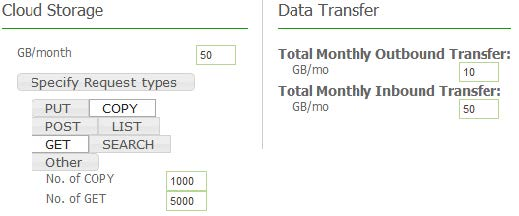
\includegraphics[width=\textwidth,keepaspectratio]{Figures/system/CloudRecommender/ServiceSelectionTestCase.jpg}
  \caption{Service selection criteria set by business analyst.}
  \label{fig:ServiceSelectionTestCase}
\end{figure}
Suppose an enterprise wants to migrate its data to the
cloud with the aim of storing and sharing it with other branches through public cloud
storage (note that security issues are dealt within the enterprise applications). At this
stage, we assume the business analyst of the enterprise has a good estimation of the
data storage and transfer (network in/network out) requirements. By using
CloudRecommender, the analyst would like to find out which of the public cloud
providers would be most cost-effective in regards to data storage and transfer costs.
For this selection scenario, the analyst inputs the following anticipated usage
information for the storage and network services: (i) Data size of 50 GB, 1000 copy
requests and 5000 get requests and (ii) data transfer in size of 10 GB and data transfer
out size of 50 GB.

As shown in Fig. \ref{fig:ServiceSelectionTestCase}, the analyst specifies service selection criteria via the storage and network widgets. Programmatically, the above request can also be submitted via the
RESTful service interface of the CloudRecommender as shown below in Fig. \ref{fig:ExampleRESTcallGET}.

\begin{figure}[!ht]
  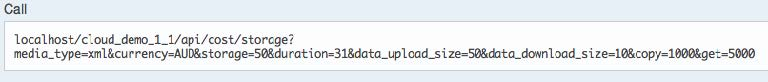
\includegraphics[width=\textwidth,keepaspectratio]{Figures/system/CloudRecommender/GET.jpg}
  \caption{An Example REST call.}
  \label{fig:ExampleRESTcallGET}
\end{figure}

Once this selection request is submitted, the controller validates and parameterizes the
criteria (user inputs). Though not shown in the above figures, the business analyst also has the
option to express whether the selection criteria should be evaluated against all the
available cloud providers or only the selected ones (e.g., Amazon, Azure, and GoGrid
only). As mentioned earlier, the application logic layer implements specialized views
and procedures for evaluating different service selection scenarios.
CloudRecommender captures and inserts multiple storage and network service
selection criteria into specialized views called "\texttt{storage\_selection\_criteria}" and
"\texttt{network\_selection\_criteria}". Aforementioned views are then joined against the
"\texttt{storage\_service\_price}" and "\texttt{network\_service\_price}" views for estimating the cost of
using the combined cloud services.

\begin{figure}[!ht]
  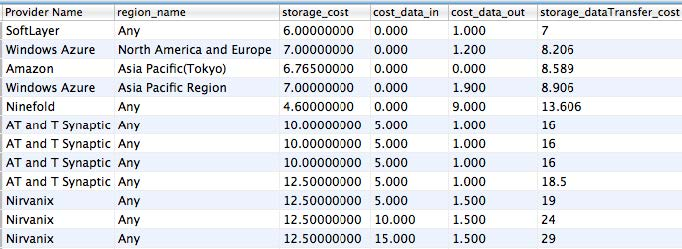
\includegraphics[width=\textwidth,keepaspectratio]{Figures/system/CloudRecommender/recommendationResults.jpg}
  \caption{Storage and network services recommendations for the business analyst selection use case.}
  \label{fig:StorageNetworkServicesRecommendations}
\end{figure}

Fig. \ref{fig:StorageNetworkServicesRecommendations} shows the result of the
selection scenario depicted in Fig. \ref{fig:ServiceSelectionTestCase}.
Results are sorted into increasing total cost order (i.e. "\texttt{storage\_dataTransfer\_cost}"
column). "Any" means the provider offers the same price for all of its regions. In the
case of SoftLayer, it charges the same price in all regions. In the case of Amazon
AWS, since it offers different prices for different regions, the enterprise may be able
to consume the same service with a cheaper price in a different region. The base
currency is USD, but since in the call the analyst had specified "currency=AUD", the
result shown is in AUD accurate to one decimal place.

\begin{figure}[!ht]
  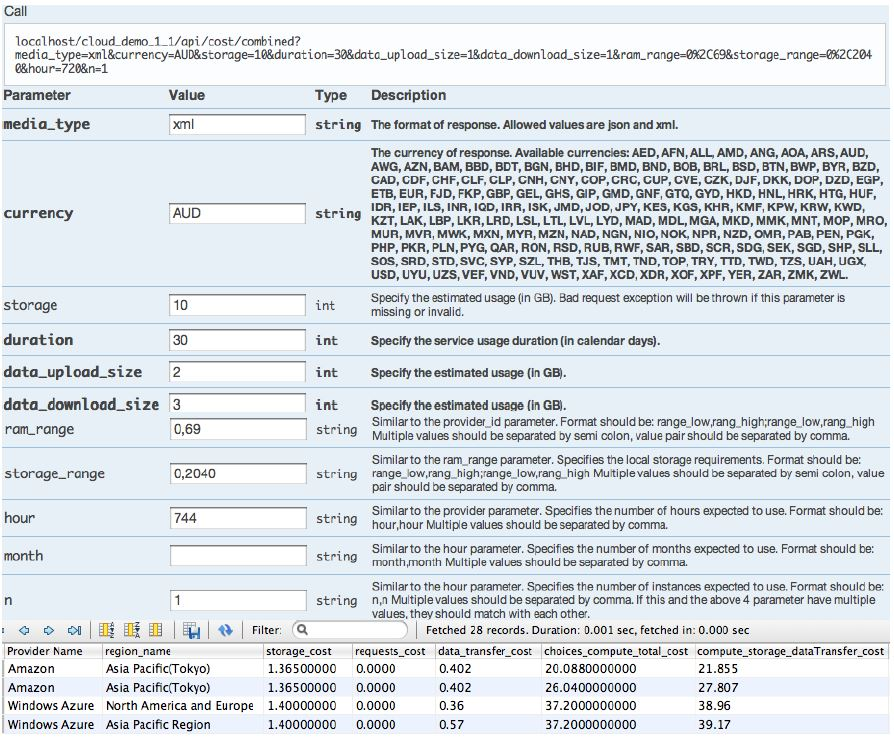
\includegraphics[width=\textwidth,keepaspectratio]{Figures/system/CloudRecommender/ResultOfSelectionForComputeStorageNetwork.jpg}
  \caption{Result of selection process for Compute, Storage and network services}
  \label{fig:ResultOfSelectionForComputeStorageNetwork}
\end{figure}

Fig. \ref{fig:ResultOfSelectionForComputeStorageNetwork} shows another
example which selects compute, storage, and network using the RESTful API. The
selection criteria include 1 compute service instance (shown as "n=1"):
0<Ram<=69, 0<=local storage<=2040, number of hours to be used per month 744.
The selection results are displayed at the end of the figure.

Due to high inter-cloud data transfer cost overhead and communication delay, our
recommender logic does not consider the combination of services from multiple
providers. For example, the CloudRecommender will not select and combine compute
service from Amazon with storage service from Azure. 
Similarly, some provider charge for data transfer across their
own services that are hosted at different regions. For example, data transferred
between Amazon services in different regions are charged as “Internet Data Transfer”
on both sides of the transfer. We currently choose to put all services in the same
region. In future we may extend our recommendation logic to allow users to choose
between different regions for each service type (if necessary). Additionally providers
often offer discounted price for higher usage, keeping all data together means higher
usage which can consume a cheaper price tier. Network services are always bundled
with either compute or storage service as it is impossible to consume other services
without incurring network costs.

\subsection{Case Studies}
\label{sec:case_studies}
Gaia is a global space astrometry mission with a goal of making the largest, most precise three-dimensional map of our Galaxy by surveying more than one billion starts. For the amount of images produced by the satellite (1 billion stars $\times$ 80 observations $\times$ 10 readouts), if it took one millisecond to process one image, it would take 30 years of data processing time on a single processor. Luckily the data does not need to be processed continuously, every 6 months they need to process all the observations in as short a time as possible (typically two weeks) \cite{GaiaCaseStudy}.
Hypothetically speaking say they choose to use 120 high CPU and memory VMs. The example search via CloudRecommender is shown in Fig. \ref{fig:GaiaCaseStudy}. With each VM running 12 threads, there were 1440 processes working in parallel. This will reduce the processing time to less than 200 hours (about a week).

\begin{figure}
  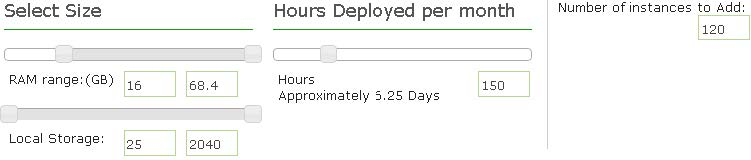
\includegraphics[width=\textwidth,keepaspectratio]{Figures/system/CloudRecommender/GaiaCaseStudy.jpg}
  \caption{Example input parameter values.}
  \label{fig:GaiaCaseStudy}
\end{figure}

In this case since data can be moved into/out of the cloud in bulk periodically, FedEx hard drive may be preferred over transferring data over the internet.

Promotional offers may not matter much in this case compare to the huge time and capital investment savings. But it makes a big difference for small business (or start ups) running a website.

Another example usage is sites with large continuous data input and processing need like Yelp. Everyday Yelp generates and stores around 100GB of logs and photos; runs approximately 200 MapReduce jobs and processing 3TB of data \cite{YelpCaseStudy}. Yelp.com has more than 71 million monthly unique visitors \cite{YelpFactsheet}. The average page size of a typical website is about 784 kB \cite{Pingdom}. So the estimated data download traffic is about 51TB per month if every unique user only views one page once a month. Fig. \ref{fig:YelpCaseStudy} shows a sample search for the above mentioned scenario.

\begin{figure}
  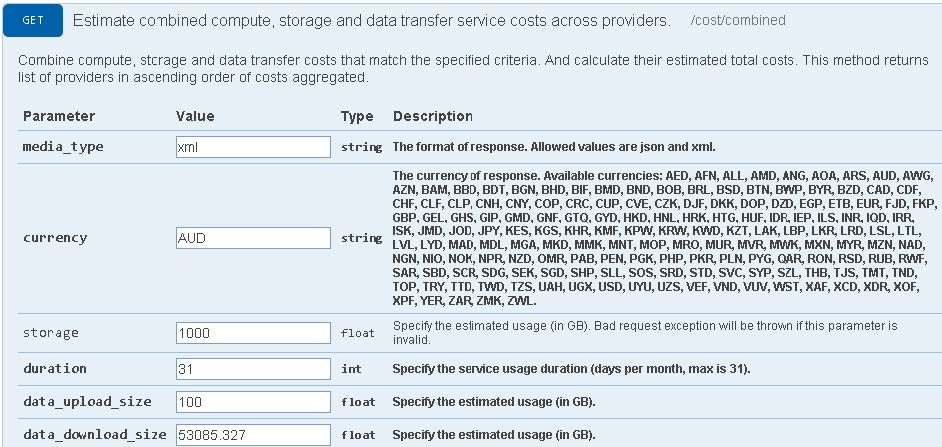
\includegraphics[width=\textwidth,keepaspectratio]{Figures/system/CloudRecommender/YelpCaseStudy.jpg}
  \caption{Example parameters for REST API.}
  \label{fig:YelpCaseStudy}
\end{figure}

% \includepdf[pages=2-,pagecommand={}]{papers/3.pdf}
